\documentclass[a4paper,11pt]{article}

% Page geometry
\usepackage[margin=2.2cm,top=2.5cm,bottom=2.8cm]{geometry}

% Essential packages
\usepackage[utf8]{inputenc}
\usepackage[T1]{fontenc}
\usepackage{microtype}

% COLORS — U-tad brand palette
\usepackage[dvipsnames]{xcolor}
\definecolor{background}{HTML}{ffffff}
\definecolor{utadblue}{HTML}{0033A0}
\definecolor{utaddark}{HTML}{001F66}
\definecolor{utadlight}{HTML}{E8EDF8}
\definecolor{utadrow}{HTML}{F2F5FC}
\definecolor{textmuted}{HTML}{5a5a5a}
\definecolor{grid}{HTML}{d0d8e8}
\definecolor{accent}{HTML}{0033A0}

% -----------------------------------------------------------------------
% FONT — full sans-serif via TeX Gyre Heros (Helvetica clone, in TeX Live)
% -----------------------------------------------------------------------
\usepackage{tgheros}
\renewcommand{\familydefault}{\sfdefault}
\usepackage{microtype}

% Tables
\usepackage{booktabs}
\usepackage{siunitx}
\usepackage{array}
\usepackage{colortbl}

% Float placement control
\usepackage{float}

% Bibliography
\usepackage[style=numeric,autocite=superscript,backend=biber,sorting=none]{biblatex}
\addbibresource{./report.bib}

% References helper
\makeatletter
\newcommand*{\sref}[1]{%
  \hyperref[{#1}]{%
    \color{accent}\textsuperscript{\ref*{#1}}%
  }%
}
\makeatother

% Graphics and links
\usepackage{graphicx}
\usepackage{hyperref}
\hypersetup{
  colorlinks=true,
  linkcolor=accent,
  urlcolor=accent,
  citecolor=accent,
  pdfborder={0 0 0},
  pdftitle={Firearm Violence and Legislation in the US},
  pdfauthor={Itziar Morales Rodr\'{i}guez}
}

% -----------------------------------------------------------------------
% HEADERS / FOOTERS
% -----------------------------------------------------------------------
\usepackage{fancyhdr}
\pagestyle{fancy}
\fancyhf{}
\fancyhead[L]{\small\color{textmuted} Firearm Violence and Legislation in the US}
\fancyfoot[R]{\small\color{textmuted}\thepage}
\fancyfoot[L]{\small\color{textmuted} U-tad}
\renewcommand{\headrulewidth}{0.6pt}
\renewcommand{\headrule}{\color{grid}\hrule height 0.6pt}
\renewcommand{\footrulewidth}{0.4pt}
\renewcommand{\footrule}{\color{grid}\hrule height 0.4pt}

% -----------------------------------------------------------------------
% SECTION HEADINGS
% -----------------------------------------------------------------------
\usepackage{titlesec}
\titleformat{\section}
  {\large\bfseries\color{utaddark}}
  {\color{accent}\thesection}{0.6em}{}
  [\vspace{0.15em}{\color{grid}\titlerule[0.5pt]}]
\titleformat{\subsection}
  {\normalsize\bfseries\color{utaddark}}
  {\thesubsection}{0.5em}{}
\titleformat{\subsubsection}
  {\small\bfseries\color{accent}}
  {\thesubsubsection}{0.5em}{}
\titlespacing*{\section}{0pt}{1.8em}{0.8em}
\titlespacing*{\subsection}{0pt}{1.3em}{0.5em}
\titlespacing*{\subsubsection}{0pt}{1em}{0.4em}

% Table style helpers
\arrayrulecolor{grid}
\setlength{\arrayrulewidth}{0.5pt}

% -----------------------------------------------------------------------
% ENUMERATIONS
% -----------------------------------------------------------------------
\usepackage{enumitem}
\setlist[itemize]{leftmargin=*,itemsep=2pt,parsep=0pt}
\setlist[enumerate]{leftmargin=*,itemsep=2pt,parsep=0pt}

% -----------------------------------------------------------------------
% PROMPT / RESPONSE BOX
% -----------------------------------------------------------------------
\usepackage{mdframed}
\mdfdefinestyle{promptbox}{
  backgroundcolor=utadlight,
  linecolor=accent,
  linewidth=1.4pt,
  leftline=true, rightline=false, topline=false, bottomline=false,
  innerleftmargin=10pt, innerrightmargin=8pt,
  innertopmargin=6pt, innerbottommargin=6pt,
  skipabove=6pt, skipbelow=6pt
}
\renewenvironment{quote}
  {\begin{mdframed}[style=promptbox]\small}
  {\end{mdframed}}

% Verbatim
\usepackage{fancyvrb}
\RecustomVerbatimEnvironment{verbatim}{Verbatim}{fontsize=\small}

% TikZ for title page
\usepackage{tikz}
\usetikzlibrary{calc}

% ======================================================================
\begin{document}
\pagecolor{background}\color{black}

% ======================================================================
% TITLE PAGE
% ======================================================================
\begin{titlepage}
	\begin{tikzpicture}[remember picture, overlay]
		\fill[utaddark] (current page.north west)
		rectangle ($(current page.north east) + (0,-3.0cm)$);
		\fill[accent] ($(current page.north west) + (0,-3.0cm)$)
		rectangle ($(current page.north east) + (0,-3.35cm)$);
		\fill[utadlight] (current page.south west)
		rectangle ($(current page.south east) + (0,1.4cm)$);
		\fill[accent] ($(current page.south west) + (0,1.4cm)$)
		rectangle ($(current page.south east) + (0,1.1cm)$);
	\end{tikzpicture}

	\vspace*{0.6cm}
	\begin{center}
		
\includegraphics[height=1.9cm]{./assets/U-tad-logo.jpg}
	\end{center}

	\vspace*{3.2cm}
	\begin{center}
		{\fontsize{26}{32}\selectfont\bfseries\color{utaddark}
			Firearm Violence and Legislation\\[0.25em]
			in the United States}\\[0.5em]
		{\fontsize{16}{22}\selectfont\color{accent}
		Data Visualization Report}\\[2.0em]
		{\color{grid}\rule{0.55\textwidth}{0.8pt}}\\[1.8em]
		{\large\color{black} Itziar Morales Rodr\'{i}guez}\\[0.6em]
		{\normalsize\color{textmuted} Data Visualization --- U-tad}\\[0.4em]
		{\normalsize\color{textmuted}\today}
	\end{center}
	\vfill
	\vspace{1.0cm}
\end{titlepage}

% ======================================================================
\tableofcontents
\newpage

% ======================================================================
\section{Introduction}
% ======================================================================

\par
This project studies the relationship between firearm laws and gun violence in
the United States from 1976 to 2023. Estimated household gun ownership is
included as background context, but it is not treated as the main explanatory
factor. Some countries, such as Finland and Switzerland, show that high gun
ownership can exist alongside relatively low gun violence. For that reason,
this project focuses mainly on whether the strength and type of state firearm
laws are associated with lower firearm homicide rates, and whether changes in
those laws are followed by changes in a state's level of gun violence.

\subsection{Methodology}

\par
The project was developed through the following steps:
\begin{enumerate}
	\item Select the datasets and plan the join strategy
	\item Explore the data outside Tableau
	\item Define the research questions
	\item Choose chart types that answer each question clearly
	\item Connect the data sources and create the required calculated fields in Tableau
	\item Add Tableau features such as parameters, sets, filters, actions, and tooltips
	\item Build dashboards for interactive storytelling
	\item Use AI only for repetitive or mechanical tasks
	      (see Section~\ref{sec:ai})
\end{enumerate}

\subsection{Sources}

\par
The project uses several types of sources:

\begin{itemize}
	\item Official dataset documentation and codebooks~\autocite{ownershipproxy,statefirearmlaw}
	\item Harvard Dataverse and Tufts CTSI metadata~\autocite{kang2023,statefirearmlaw}
	\item Academic literature on firearm ownership proxies~\autocite{extendingfss,kang2023}
	\item Academic literature on the effects of gun laws~\autocite{kopernij1999,koper2004,donohue2022}
	\item Tableau official documentation~\autocite{tableau}
	\item Lecture notebooks and course materials
	\item AI assistance, declared in Section~\ref{sec:ai}
\end{itemize}

\par
All sources are referenced in the bibliography. When AI was used, the model and
prompt are stated explicitly in the report.

\subsection{AI Usage Declaration}\label{sec:ai}

\par
AI was used only for repetitive, mechanical, or formatting-related tasks.
All output was reviewed before being included. AI did not produce the
analytical conclusions, the Tableau visualizations, or the interpretation of
the results. In all cases, the model used was \textbf{Claude Sonnet 4.6},
accessed through the Perplexity AI assistant. The exact prompts and short
response summaries are included where relevant, and Table~\ref{tab:ai}
provides an overview.

\begin{table}[H]
	\centering
	\renewcommand{\arraystretch}{1.35}
	\begin{tabular}{p{8.0cm} p{3.6cm} p{1.6cm}}
		\toprule
		\rowcolor{utaddark}
		\color{white}\textbf{Task}               &
		\color{white}\textbf{Model}              &
		\color{white}\textbf{Section}                                                      \\
		\midrule
		\rowcolor{utadrow}
		Dataset research and pairing strategy    & Claude Sonnet 4.6 & \ref{sec:datasets}  \\
		State-abbreviation calculated field      & Claude Sonnet 4.6 & \ref{sec:viz:q1}    \\
		\rowcolor{utadrow}
		Document labelling and cross-referencing & Claude Sonnet 4.6 & \ref{sec:ai:labels} \\
		Report structuring and LaTeX formatting  & Claude Sonnet 4.6 & \ref{sec:ai:latex}  \\
		\rowcolor{utadrow}
		Supplementary chart generation           & Claude Sonnet 4.6 & \ref{sec:viz:q3}    \\
		\bottomrule
	\end{tabular}
	\caption{AI usage index}
	\label{tab:ai}
\end{table}

\subsubsection{Document Labelling and Cross-Referencing}\label{sec:ai:labels}

\par
Adding labels and references across a long LaTeX document is repetitive and
easy to get wrong. This made it a suitable task for AI support, since it did
not require analytical judgement.

\begin{quote}
	\textbf{Prompt:} \textit{Add labels to questions Q1, Q2 and Q3 in the document
		and reference those labels whenever those questions are referenced in the
		document.}
\end{quote}

\begin{quote}
	\textbf{Response summary:} Added \texttt{\textbackslash label\{q1\}},
	\texttt{\textbackslash label\{q2\}}, and \texttt{\textbackslash label\{q3\}}
	to the question headings, then inserted matching cross-references in the
	question list, conclusions, and visualization summary table.
\end{quote}

\subsubsection{Report Structuring and LaTeX Formatting}\label{sec:ai:latex}

\par
AI was also used for LaTeX structure, figure placement, and page breaks.
These are technical formatting tasks and do not affect the interpretation of
the data.

\begin{quote}
	\textbf{Prompt:} \textit{For visualizations, make it so each of them is on a
		different page alongside with their text section, so page breaks are consistent
		and it doesn't break in weird places.}
\end{quote}

\begin{quote}
	\textbf{Response summary:} Added \texttt{\textbackslash usepackage\{float\}},
	inserted \texttt{\textbackslash newpage} before each visualization subsection,
	and changed figure placement from \texttt{[h]} to \texttt{[H]} so figures stay
	in the intended position.
\end{quote}

% ======================================================================
\section{Datasets}\label{sec:datasets}
% ======================================================================

\par
This project uses two public datasets. Both are available online and have a
state-year structure, which makes them suitable to combine in Tableau. The
first dataset was chosen independently. AI was then used to help identify a
second dataset that matched it well in scope and format.

\begin{quote}
	\textbf{Prompt:} \textit{I already have a state-year level dataset on
		estimated household gun ownership in the US. I need a second dataset that
		contains information about firearm legislation on a state-year basis so I
		can join them easily. What publicly available datasets would you recommend?}
\end{quote}

\begin{quote}
	\textbf{Response summary:} Recommended the Tufts CTSI State Firearm Law
	Database because it tracks firearm laws by state and year, matches the grain
	of the ownership proxy dataset, and is widely used in public health research.
\end{quote}

\subsection{Dataset 1: Firearm Suicide Proxy for Household Gun Ownership, 1949--2023}

\par
The first dataset\autocite{ownershipproxy} is a state-year level proxy for
household gun ownership in the United States. Direct state-level gun ownership
data is not publicly available, so this dataset uses the firearm suicide proxy
method: the share of suicides committed with a firearm (FSS) is used as an
indirect estimate of household gun prevalence. The dataset is hosted on Harvard
Dataverse.

\begin{itemize}
	\item \textbf{Source}: Harvard Dataverse, Kang et al.\autocite{kang2023}
	\item \textbf{Grain}: One row per U.S. state per year
	\item \textbf{Key columns}: State, Year, FSS, firearm suicides, total suicides,
	      firearm homicide rate, total homicides, population
	\item \textbf{Date span}: 1949--2023 (75 years, 50 states + D.C.)
	\item \textbf{Format}: Comma-separated values (\texttt{.csv})
\end{itemize}

\par
This dataset was chosen because it gives a long-term, population-adjusted,
and widely used measure of gun prevalence. FSS is not a direct count of guns,
but it is a common proxy in public health and policy research\autocite{extendingfss}.
In this project, FSS is used only as contextual background in the scatter plot.
The main outcome variable is firearm homicide rate.

\subsection{Dataset 2: State Firearm Law Database, 1976--2024}

\par
The second dataset\autocite{statefirearmlaw} is maintained by the State
Firearm Law Research Group at Tufts University. It records whether 72 firearm
law provisions were in effect in each U.S. state for every year from 1976 to
2024.

\begin{itemize}
	\item \textbf{Source}: Tufts CTSI --- State Firearm Law Database\autocite{statefirearmlaw}
	\item \textbf{Grain}: One row per U.S. state per year
	\item \textbf{Key columns}: State, Year, 72 binary law indicators,
	      such as permit requirements, background checks, waiting periods,
	      stand-your-ground laws, and child access prevention laws
	\item \textbf{Date span}: 1976--2024
	\item \textbf{Format}: Excel (\texttt{.xlsx})
\end{itemize}

\par
This dataset was chosen because it provides a yearly record of state firearm
laws over a long period. That makes it useful for studying whether changes in
legislation are associated with changes in gun violence. It is also widely used
in academic public health research\autocite{statefirearmlaw}.

\subsection{Join Strategy}

\par
The two datasets were connected in Tableau using a \textbf{relationship} on
\texttt{state} and \texttt{year}. The relationship was set to
\textbf{many-to-many} with \textbf{some records match} referential integrity
on both sides. This setup is appropriate because both tables have the same
state-year grain, and neither one acts as a separate dimension table. It also
allows Tableau to aggregate each table first and then combine the results,
which helps avoid row duplication. Because the two datasets overlap only from
1976 to 2023, that is the final analysis period used in the project.

\subsection{Analysis}

\par
Before connecting the data in Tableau, both files were checked to understand
their structure, labels, and possible issues. The main observations were:

\begin{itemize}
	\item Both datasets use the same full state names, so they can be joined on state
	\item The ownership proxy dataset already includes several rate variables
	\item The firearm law dataset includes 72 binary law fields and a total law count field (\texttt{lawtotal})
	\item Both datasets overlap for the years 1976--2023
\end{itemize}

\subsection{Processing}

\par
The raw data files were used directly in Tableau. No external cleaning,
renaming, or deduplication was needed. The only structural adjustment was to
exclude the District of Columbia, because it appears in the ownership dataset
but not in the firearm law dataset. All visualizations were also limited to the
years 1976--2023, which is the period covered by both sources.

\subsection{Research Questions}

\par
Three research questions were defined after the initial data exploration:

\begin{enumerate}
	\item Is a state's firearm homicide rate associated with the number
	      and type of firearm laws it has in place?\sref{q1}
	\item How have firearm homicide rates changed over time depending on
	      the firearm laws passed in each state, whether measured by
	      the quantity of laws or by the type of laws?\sref{q2}
	\item For a specific state, does passing more firearm laws correspond
	      to a reduction in firearm homicide rates, and how does this
	      affect its ranking relative to other states?\sref{q3}
\end{enumerate}

\subsubsection{Question 1: Homicide Rates and the Law Landscape}\label{q1}

\par
Q1 is the starting point of the analysis. Before looking at changes over time,
it is useful to see whether a cross-sectional pattern already exists. In other
words, do states with more laws, or different types of laws, tend to have lower
firearm homicide rates? FSS is included only to give background context about
estimated ownership, not as an outcome or a direct cause.

\subsubsection{Question 2: Homicide Trends by Law Profile Over Time}\label{q2}

\par
Q2 builds on Q1 by adding the time dimension. States are grouped by their law
profile, either by quantity tier or by law type category
(see Section~\ref{sec:lawcat}). This makes it possible to compare how firearm
homicide rates changed over time across different groups of states.

\subsubsection{Question 3: State-Level Law History and Homicide Standing}\label{q3}

\par
Q3 moves from the national picture to the state level. It lets the viewer focus
on one state and explore how its law history relates to its firearm homicide
standing compared with other states. This makes the analysis more personal and
more interactive, while still staying connected to the broader patterns shown
in Q1 and Q2.

% ======================================================================
\section{Visualization Prep}
% ======================================================================

\par
Before building the charts in Tableau, several design decisions were made so
the visualizations would be clear, consistent, and aligned with the analysis.

% -----------------------------------------------------------------------
\subsection{Storytelling}
% -----------------------------------------------------------------------

\par
The project follows a four-act structure. Act~1 introduces the geographic and
cross-sectional view by showing where firearm homicide is highest and how this
relates to the law landscape. Act~2 adds time, showing how homicide trends
change across the law categories defined in Section~\ref{sec:lawcat}. Act~3
narrows the focus to individual states, linking each state's law history to its
position relative to the rest of the country. Act~4 looks more closely at the
selected law groups and compares their average homicide trends.

% -----------------------------------------------------------------------
\subsection{Law Categorization}\label{sec:lawcat}
% -----------------------------------------------------------------------

\par
Two grouping systems are used throughout the visualizations. A shared
parameter allows the viewer to switch between them.

\par
\textbf{By quantity} --- states are grouped by their total law count
(\texttt{lawtotal}) into three levels:

\begin{itemize}
	\item \textbf{Low}
	\item \textbf{Medium}
	\item \textbf{High}
\end{itemize}

\par
\textbf{By type} --- instead of comparing all 72 laws, the analysis focuses on
a smaller subset: the three most common laws (``Popular'') and the three laws
with the strongest evidence base in the literature (``Evidence-Based''). States
are then placed into four categories depending on whether they have at least
two laws from either group:

\begin{itemize}
	\item \textbf{Weak} --- fewer than two Popular laws and fewer than two Evidence-Based laws
	\item \textbf{Popular} --- at least two Popular laws, but fewer than two Evidence-Based laws
	\item \textbf{Evidence} --- at least two Evidence-Based laws, but fewer than two Popular laws
	\item \textbf{Both} --- at least two laws from each group
\end{itemize}

% -----------------------------------------------------------------------
\subsection{Colors and Themes}\label{colors}
% -----------------------------------------------------------------------

\par
Colors were chosen to keep the charts clear and avoid adding political bias.

\begin{itemize}
	\item \textbf{Neutral colors} were used to avoid suggesting a political position.
	      Grey was used for states with weaker law profiles or less notable change.
	\item \textbf{Orange gradient} was used for value scales such as firearm homicide
	      rate, where darker shades represent higher values.
	\item \textbf{Gridlines} were kept minimal so attention stays on the data rather than the chart frame.
\end{itemize}

% ======================================================================
\section{Visualizations}
% ======================================================================

\par
All visualizations follow the same color logic described in Section~\ref{colors}
and use the law categories defined in Section~\ref{sec:lawcat}.

% --- Q1 -----------------------------------------------------------------
\newpage
\subsection{Q1 -- Homicide Rates and the Law Landscape}\label{sec:viz:q1}

\par
Two charts answer Q1\sref{q1}. The first is a \textbf{choropleth map}
(Figure~\ref{fig:q1chart1}) showing firearm homicide rate by state for a
selected year. The map uses an orange gradient, where darker states have
higher rates. A \textbf{parameter} controls the year, and a \textbf{calculated
field} provides the two-letter state abbreviations shown on the map.

\par
The calculated field for state abbreviations was created with AI support
(Claude Sonnet 4.6; see Section~\ref{sec:ai}). Writing all 50 cases by hand
would have been repetitive and easy to mistype. The prompt and response are
shown below (Prompt~\ref{prompt:abbr}).

\begin{quote}\label{prompt:abbr}
	\textbf{Prompt:} \textit{Generate a Tableau calculated field using a CASE
		statement that maps each U.S.\ state's full name to its two-letter
		abbreviation for all 50 states. Only output the code.}
\end{quote}

\begin{quote}
	\textbf{Response:}
	\begin{Verbatim}[fontsize=\footnotesize]
		CASE [State]
		WHEN "Alabama" THEN "AL"
		WHEN "Alaska"  THEN "AK"
		...
		WHEN "Wisconsin" THEN "WI"
		WHEN "Wyoming"   THEN "WY"
		END
	\end{Verbatim}
\end{quote}

\begin{figure}[H]
	\centering
	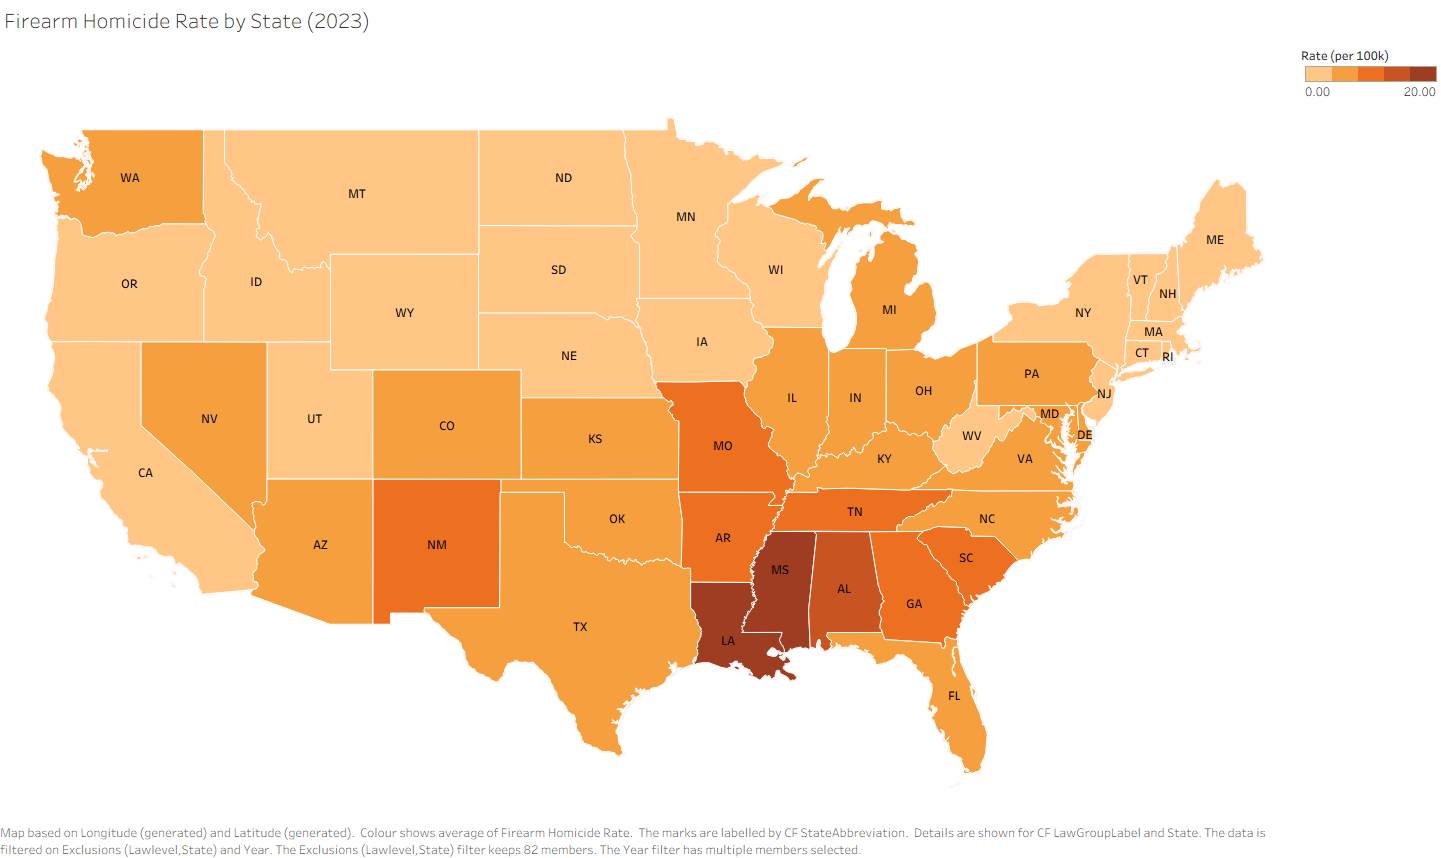
\includegraphics[width=0.95\textwidth]{../figures/Q1Chart1.png}
	\caption{Q1 -- Firearm Homicide Rate by State (Choropleth Map)}
	\label{fig:q1chart1}
\end{figure}

\par
The second chart (Figure~\ref{fig:q1chart2}) is a \textbf{scatter plot}.
Each point is a state. The X axis shows estimated gun ownership (FSS), the Y
axis shows total law count (\texttt{lawtotal}), and color reflects the selected
law profile. A \textbf{parameter} allows the viewer to switch between the
quantity-based and type-based groupings defined in Section~\ref{sec:lawcat}.

\begin{figure}[H]
	\centering
	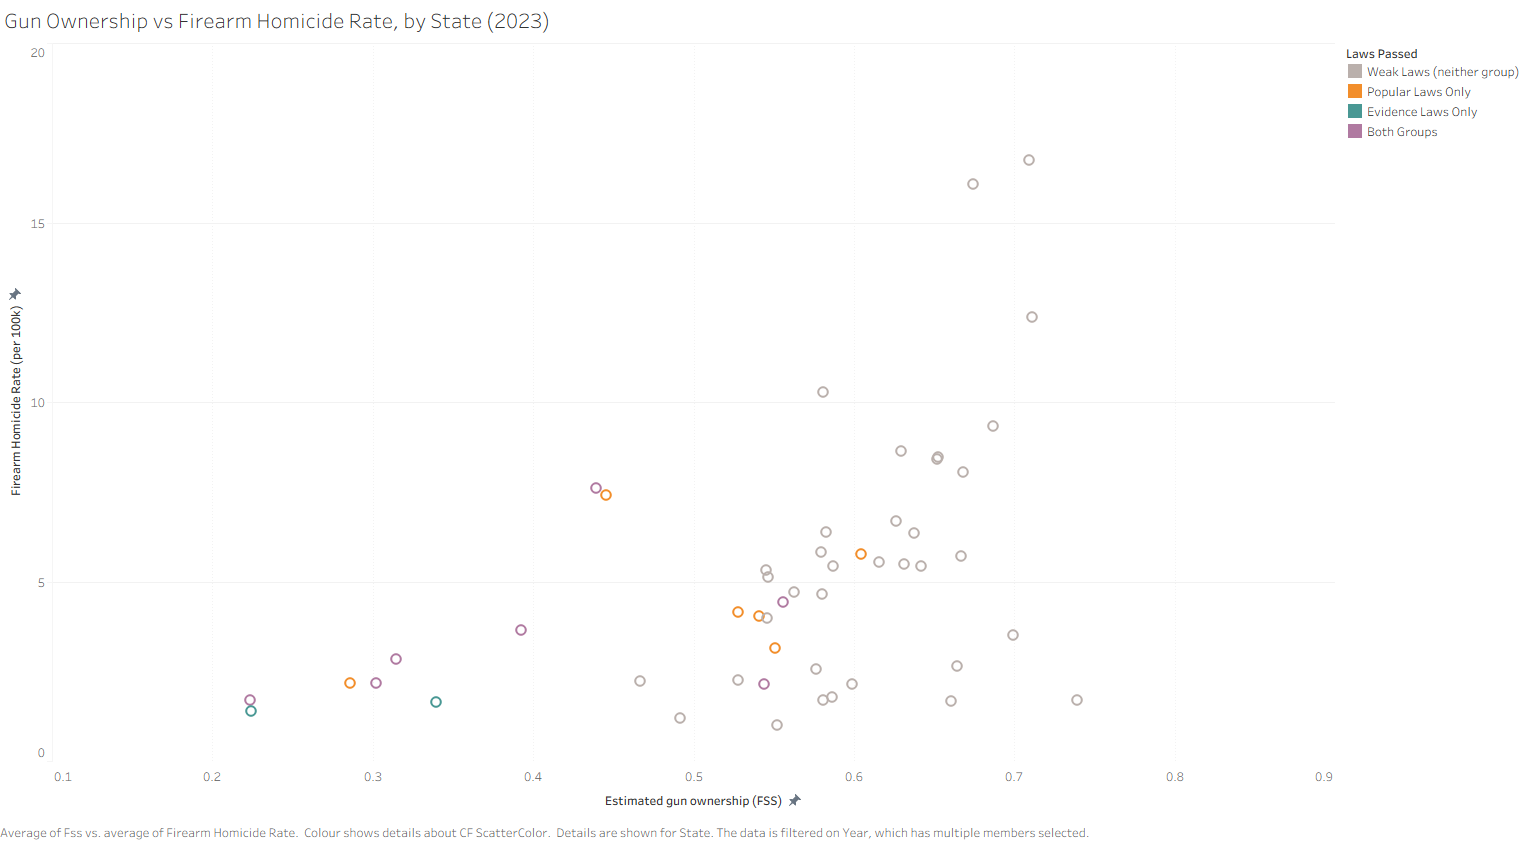
\includegraphics[width=0.95\textwidth]{../figures/Q1Chart2.png}
	\caption{Q1 -- Law Count vs.\ Estimated Gun Ownership (FSS), colored by Law Profile (Scatter Plot)}
	\label{fig:q1chart2}
\end{figure}

\textbf{Insights}: States with fewer laws tend to cluster around higher
firearm homicide rates. The FSS axis adds ownership context, but the main
focus remains on law count and law type.

% --- Q2 -----------------------------------------------------------------
\newpage
\subsection{Q2 -- Homicide Trends by Law Profile Over Time}\label{sec:viz:q2}

\par
Q2\sref{q2} is answered with an \textbf{interactive line chart}
(Figure~\ref{fig:q2chart}). The X axis shows year from 1976 to 2023, and the Y
axis shows firearm homicide rate. Each line represents a group of states based
on the active law grouping parameter, which is shared with Figure~\ref{fig:q1chart2}.
When the parameter is set to quantity, the groups are Low, Medium, and High.
When it is set to type, the groups are Weak, Popular, Evidence, and Both.
A vertical \textbf{reference line} marks notable legislative periods.

\begin{figure}[H]
	\centering
	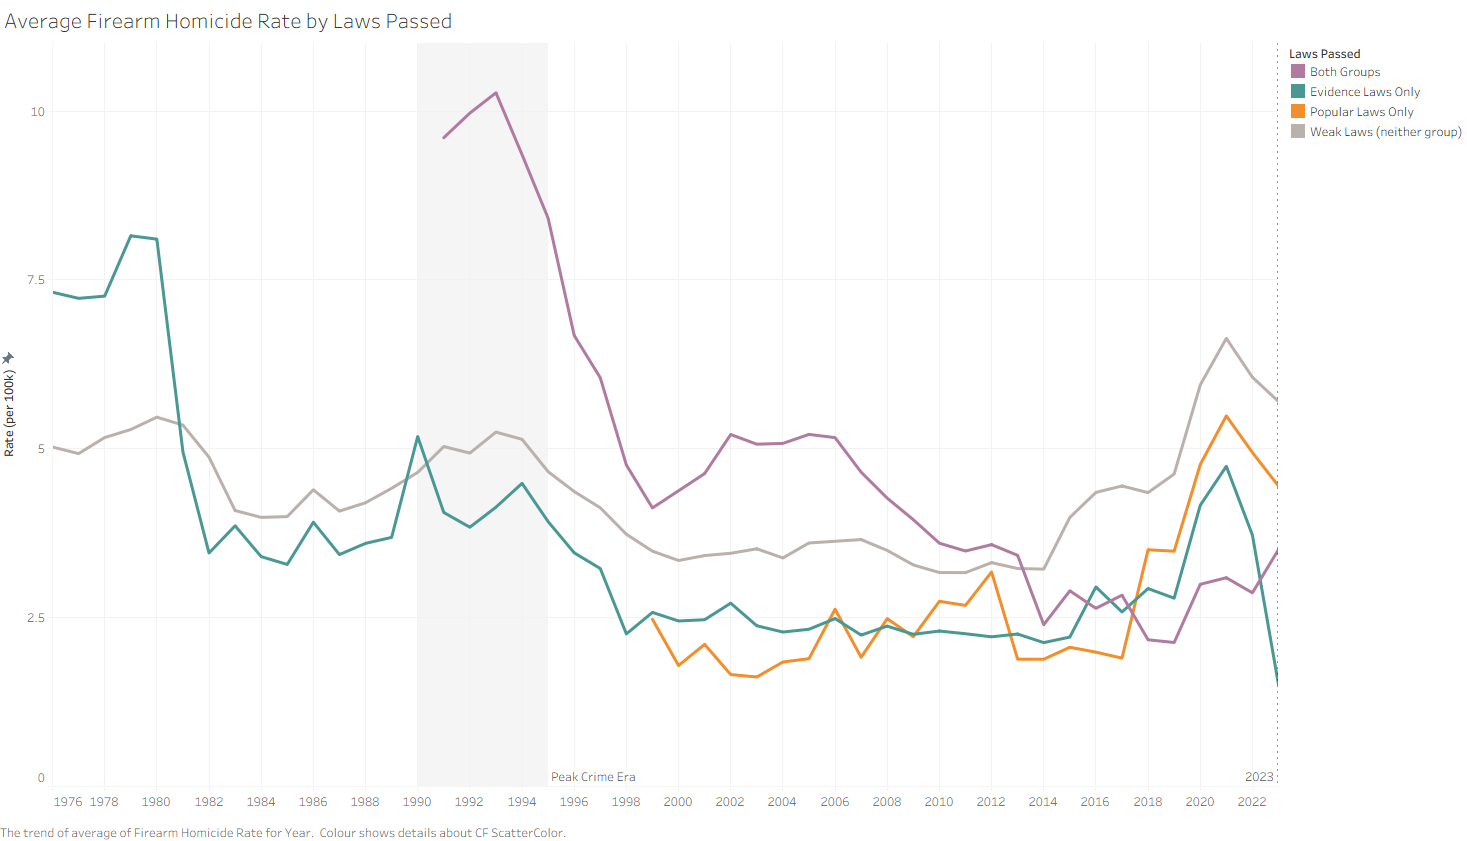
\includegraphics[width=0.95\textwidth]{../figures/Q2Chart.png}
	\caption{Q2 -- Firearm Homicide Rate Over Time by Law Profile (1976--2023)}
	\label{fig:q2chart}
\end{figure}

\textbf{Insights}: States in the higher-law groups show a clearer decline in
firearm homicide rates from the 1990s onward. The gap between groups also grows
over time, and this pattern appears under both grouping systems.

% --- Q3 -----------------------------------------------------------------
\newpage
\subsection{Q3 -- State-Level Law History and Homicide Standing}\label{sec:viz:q3}

\par
Two charts answer Q3\sref{q3}. The first (Figure~\ref{fig:q3chart1}) is a
\textbf{line chart} that shows the total number of firearm laws in effect over
time for a selected state. A \textbf{parameter} controls which state is shown.
This helps identify periods when the state's legal framework changed the most.
The second chart (Figure~\ref{fig:q3chart2}) is a \textbf{bar chart} ranking
all states by firearm homicide rate in a selected year. Bars are colored by law
category, and the selected state is highlighted with a \textbf{set}. A national
average \textbf{reference line} gives extra context. Together, these two charts
show how a state's law history relates to its position compared with other
states.

\begin{figure}[H]
	\centering
	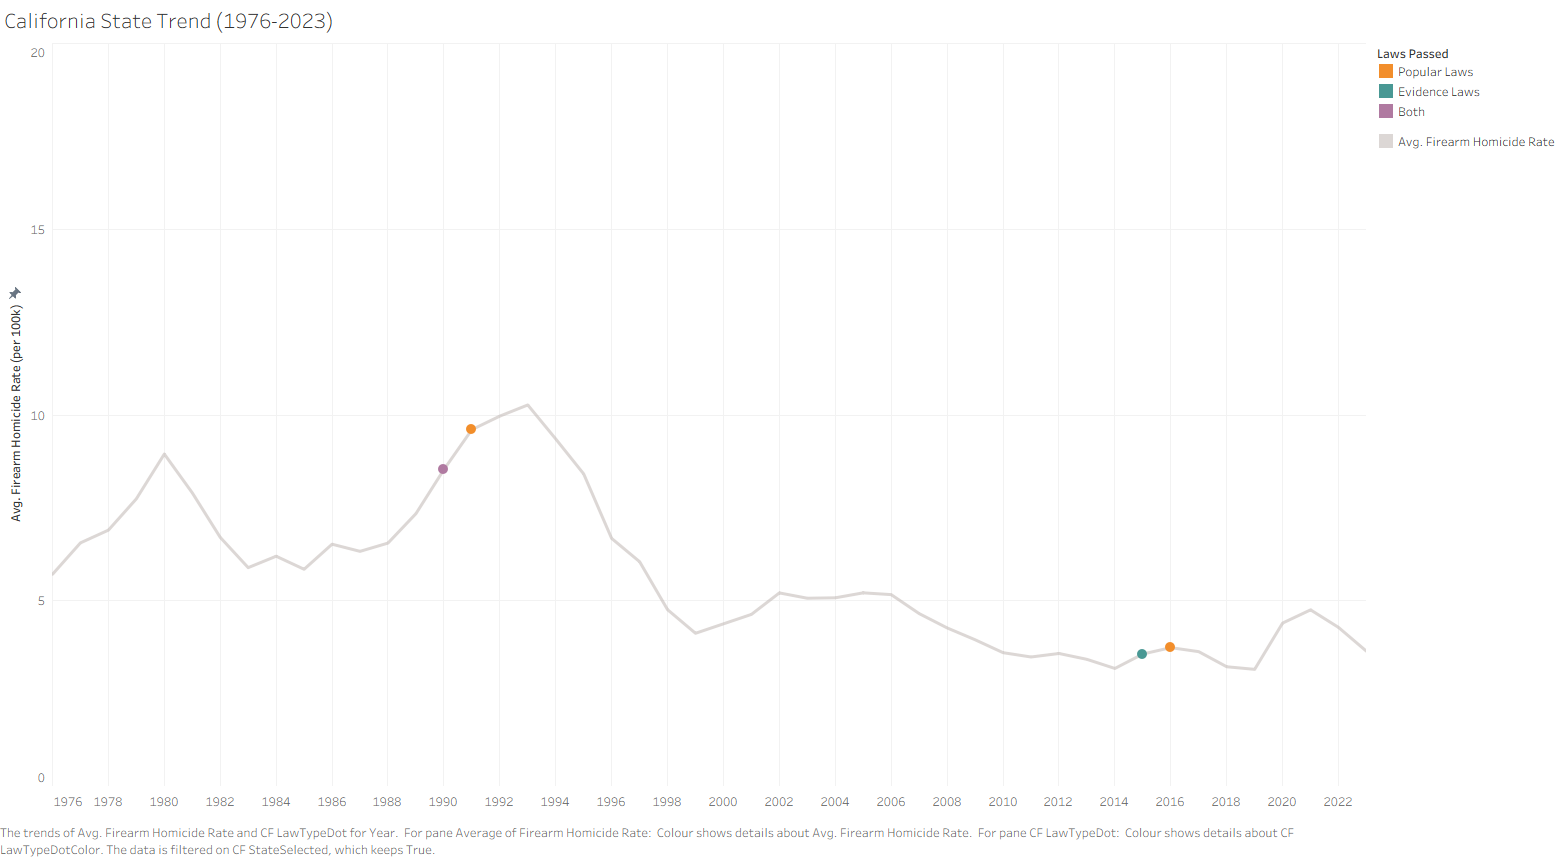
\includegraphics[width=0.95\textwidth]{../figures/Q3Chart1.png}
	\caption{Q3 -- Firearm Laws in Effect Over Time for Selected State (Line Chart)}
	\label{fig:q3chart1}
\end{figure}

\begin{figure}[H]
	\centering
	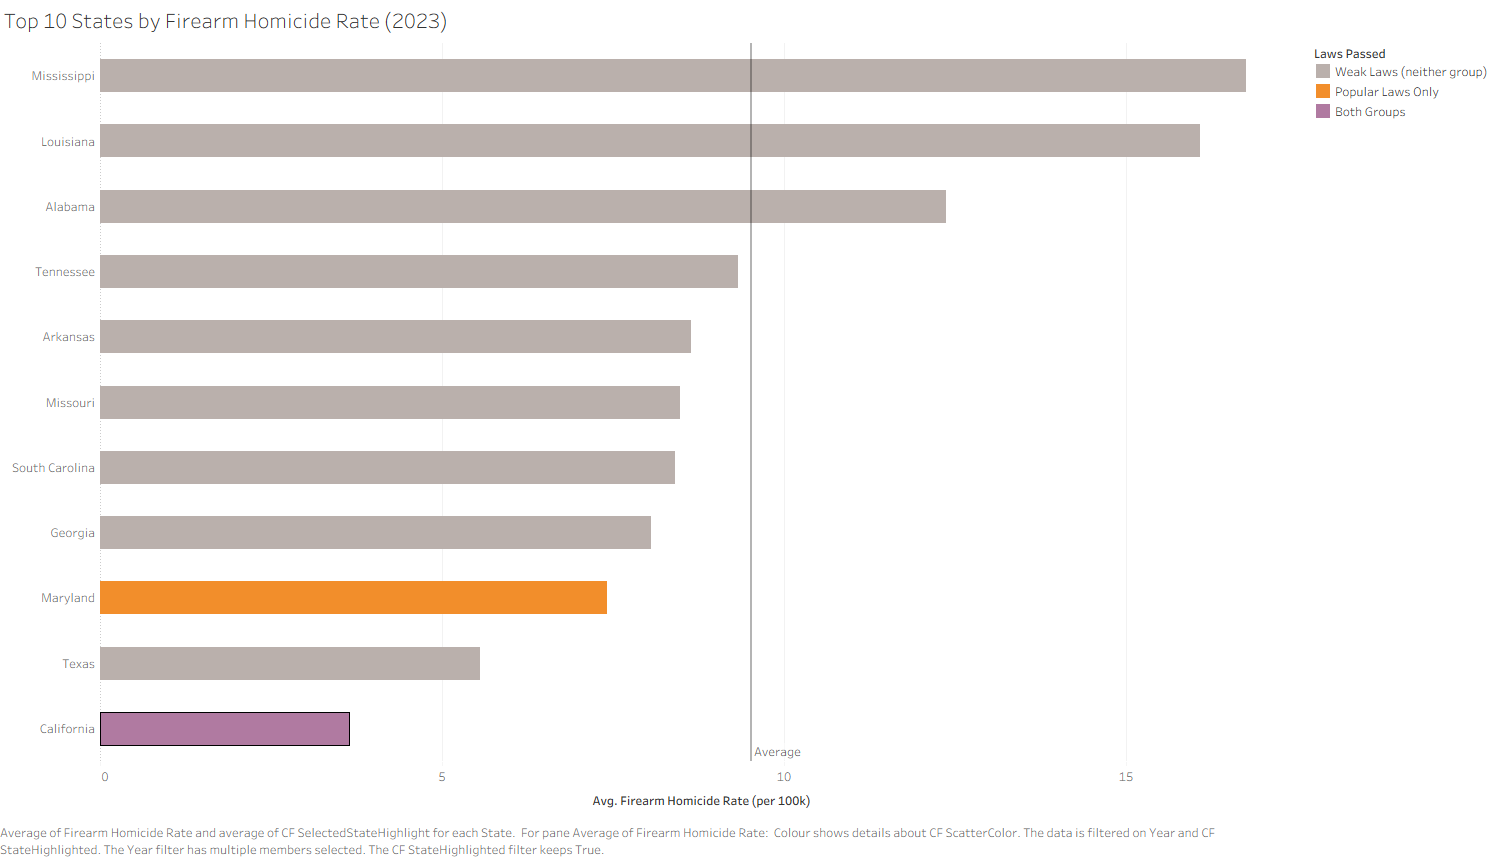
\includegraphics[width=0.95\textwidth]{../figures/Q3Chart2.png}
	\caption{Q3 -- Firearm Homicide Rate by State, Selected State Highlighted, National Average Reference Line (Bar Chart)}
	\label{fig:q3chart2}
\end{figure}

\textbf{Insights}: In several states, a steady increase in the number of laws
is associated with a better position in the homicide ranking. This pattern is
not identical in every state, so no causal claim is made.

% --- Dashboards ---------------------------------------------------------
\newpage
\subsection{Dashboards}\label{sec:dashboards}

\par
Two dashboards combine the individual charts into a more complete interactive
view.

\par
\textbf{Dashboard 1} (Figure~\ref{fig:db1}) combines the choropleth map
(Figure~\ref{fig:q1chart1}), the scatter plot (Figure~\ref{fig:q1chart2}),
and the line chart for Q2 (Figure~\ref{fig:q2chart}). It addresses Q1\sref{q1}
and Q2\sref{q2} together. A \textbf{dashboard set action} on the map highlights
the selected state in the scatter plot and updates the line chart. The shared
law-group \textbf{parameter} also changes the grouping across all three views.

\begin{figure}[H]
	\centering
	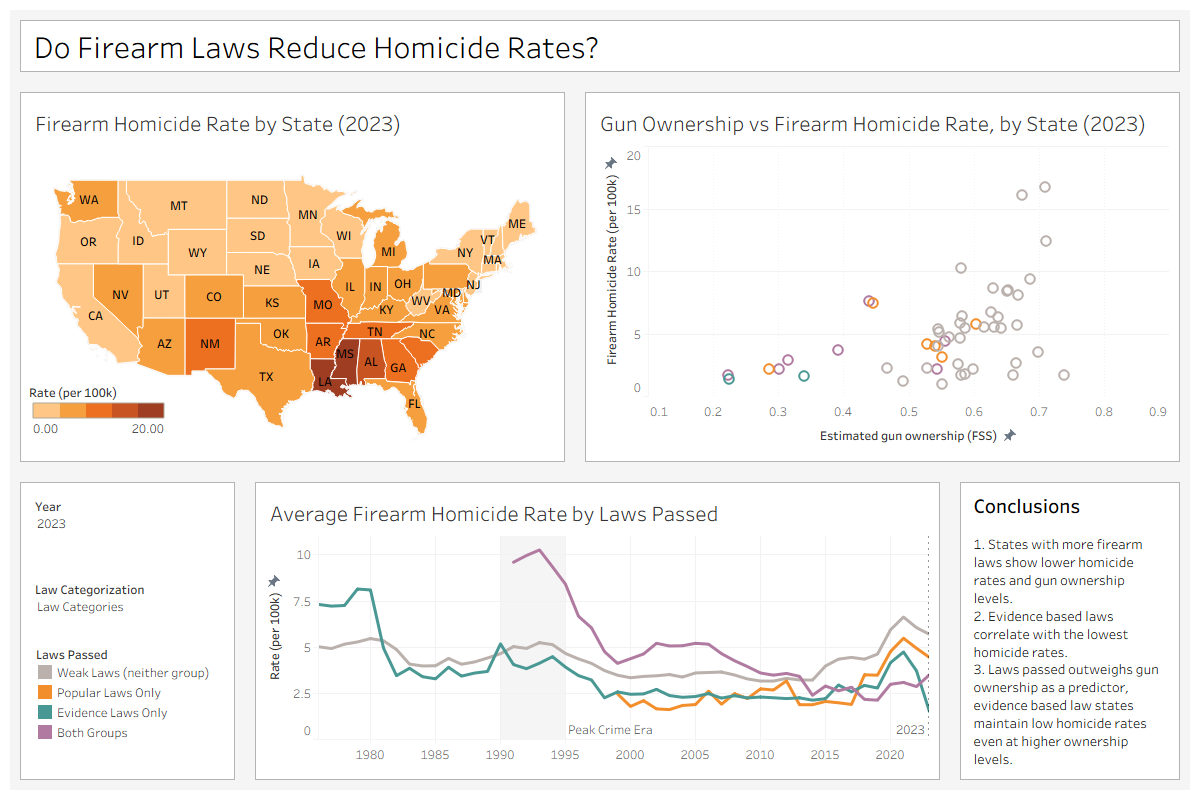
\includegraphics[width=0.95\textwidth]{../figures/Dashboard1.png}
	\caption{Dashboard 1 -- Geographic Overview, Law--Homicide Scatter, and Law Profile Trends (Q1 + Q2)}
	\label{fig:db1}
\end{figure}

\par
\textbf{Dashboard 2} (Figure~\ref{fig:db2}) focuses on Q3\sref{q3} while also
connecting back to Q1\sref{q1} and Q2\sref{q2}. It combines the choropleth map
(Figure~\ref{fig:q1chart1}), the state ranking bar chart
(Figure~\ref{fig:q3chart2}), and the state law history line chart
(Figure~\ref{fig:q3chart1}). The shared state \textbf{parameter} controls both
the line chart and the highlighted state in the ranking chart.

\begin{figure}[H]
	\centering
	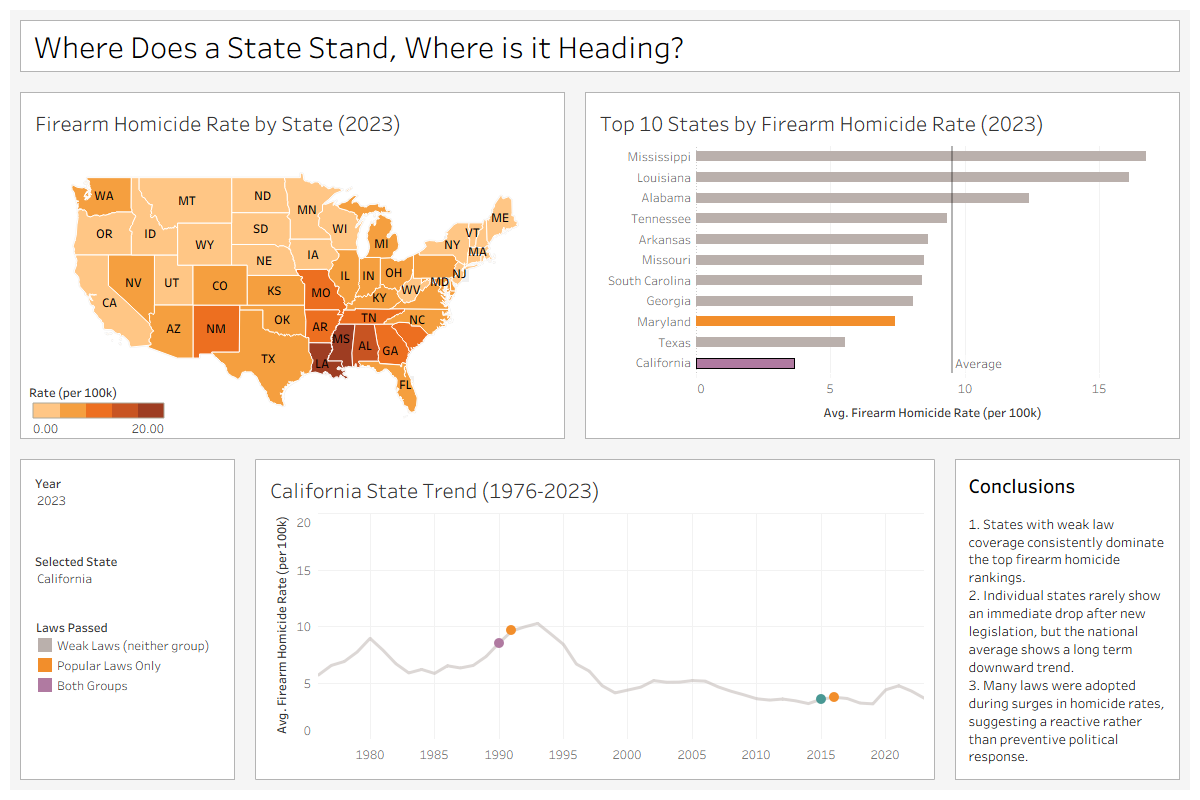
\includegraphics[width=0.95\textwidth]{../figures/Dashboard2.png}
	\caption{Dashboard 2 -- Geographic Map, State Homicide Ranking, and Selected State Law History (Q3 + Q1/Q2)}
	\label{fig:db2}
\end{figure}

% --- Summary table ------------------------------------------------------
\newpage
\subsection{Visualization Summary}

\begin{table}[H]
	\centering
	\renewcommand{\arraystretch}{1.35}
	\begin{tabular}{p{1.0cm} p{2.0cm} p{4.2cm} p{6.0cm}}
		\toprule
		\rowcolor{utaddark}
		\color{white}\textbf{Q}          &
		\color{white}\textbf{Chart}      &
		\color{white}\textbf{Chart Type} &
		\color{white}\textbf{Tableau Features}                                                                    \\
		\midrule
		\rowcolor{utadrow}
		Q1\sref{q1}                      & Fig.~\ref{fig:q1chart1}                     & Choropleth map
		                                 & Parameter, calculated field, color encoding                            \\
		Q1\sref{q1}                      & Fig.~\ref{fig:q1chart2}                     & Scatter plot
		                                 & Parameter, color encoding                                              \\
		\rowcolor{utadrow}
		Q2\sref{q2}                      & Fig.~\ref{fig:q2chart}                      & Line chart (interactive)
		                                 & Parameter, reference line                                              \\
		Q3\sref{q3}                      & Fig.~\ref{fig:q3chart1}                     & Line chart (per state)
		                                 & Parameter, filter                                                      \\
		\rowcolor{utadrow}
		Q3\sref{q3}                      & Fig.~\ref{fig:q3chart2}                     & Bar chart (comparative)
		                                 & Set, reference line, set action                                        \\
		Q1+Q2                            & Fig.~\ref{fig:db1}                          & Dashboard
		                                 & Set action, parameter, filter                                          \\
		\rowcolor{utadrow}
		Q3+Q1/Q2                         & Fig.~\ref{fig:db2}                          & Dashboard
		                                 & Parameter, set action, filter                                          \\
		\bottomrule
	\end{tabular}
	\caption{Visualization summary}
	\label{tab:summary}
\end{table}

\par
Table~\ref{tab:summary} shows the main visual elements used in the project:

\begin{itemize}
	\item Four chart types: choropleth map, scatter plot, line chart, and bar chart
	\item Tableau features such as calculated fields, parameters, sets, dashboard actions, reference lines, filters, and tooltips
	\item Two data sources connected by state and year, using two different file formats (\texttt{.csv} and \texttt{.xlsx})
\end{itemize}

% ======================================================================
\section{Conclusions}
% ======================================================================

\par
The visualizations suggest the following main patterns:

\begin{itemize}
	\item Q1\sref{q1}: States with fewer firearm laws tend to show higher firearm homicide rates in both the geographic and cross-sectional views (Figure~\ref{fig:q1chart2}).
	\item Q2\sref{q2}: States with more laws, whether measured by quantity or by type, show a stronger decline in firearm homicide rates from the 1990s onward (Figure~\ref{fig:q2chart}).
	\item Q3\sref{q3}: In several states, growth in the number of laws is associated with a better position in the homicide ranking, although this is not consistent enough to support a causal claim (Figures~\ref{fig:q3chart1} and~\ref{fig:q3chart2}).
	\item FSS is useful as background context, but the main analytical focus of the project remains the legal environment rather than ownership itself.
\end{itemize}

\par
This project also has some limitations. FSS is only a proxy for gun ownership,
not a direct measure. The analysis does not control for other factors such as
poverty or urbanization. In addition, the state-level join may hide variation
within states.

\newpage

\section{References}
\printbibliography[heading=none]

\end{document}
